\chapter{Diagram Biner Padat--Cair}\label{ch:b2:solid-liquid-diagrams}

Timah melebur pada \qty{232}{\degreeCelsius} dan timbal pada
\qty{327}{\degreeCelsius}, tetapi solder lama para teknisi listrik,
campuran keduanya, melebur pada \qty{182}{\degreeCelsius}, di bawah
keduanya. Garam yang ditaburkan di jalan mencairkan es, tetapi hanya
sampai sekitar \qty{-21}{\degreeCelsius}; pada malam yang lebih dingin,
garam itu tidak berbuat apa-apa. Sebaliknya, tembaga dan nikel bercampur
dalam perbandingan berapa pun bahkan dalam keadaan padat, dan paduannya
melebur dalam suatu rentang suhu di antara titik lebur kedua logam itu.
Diagram-diagram dalam bab ini menyatakan, untuk setiap pasangan, padatan
mana yang mengkristal dari cairan yang mendingin, pada suhu berapa, dan
dalam jumlah berapa --- pengetahuan di balik setiap pengecoran, setiap
sambungan solder, dan setiap paduan bertitik lebur rendah.

\begin{recall}
\Cref{ch:b2:chemical-potential}: \omterm{def:b2:chemical-potential:chemical-potential}{potensial kimia} sebuah komponen dalam
\omterm{def:b2:chemical-potential:ideal-mixture}{campuran ideal}, krioskopi. \Cref{ch:b2:equilibrium-shifts}: \omterm{def:b2:equilibrium-shifts:variance}{varians}.
\Cref{ch:b2:liquid-vapour-diagrams}: \omterm{def:b2:liquid-vapour-diagrams:binary-diagram}{diagram biner}, garis hubung, dan
\omterm{thm:b2:liquid-vapour-diagrams:lever}{aturan tuas}. Jilid Tahun 1: ikatan logam, paduan substitusi dan paduan
interstisi, tipe-tipe kristal.
\end{recall}

\begin{omfigure}
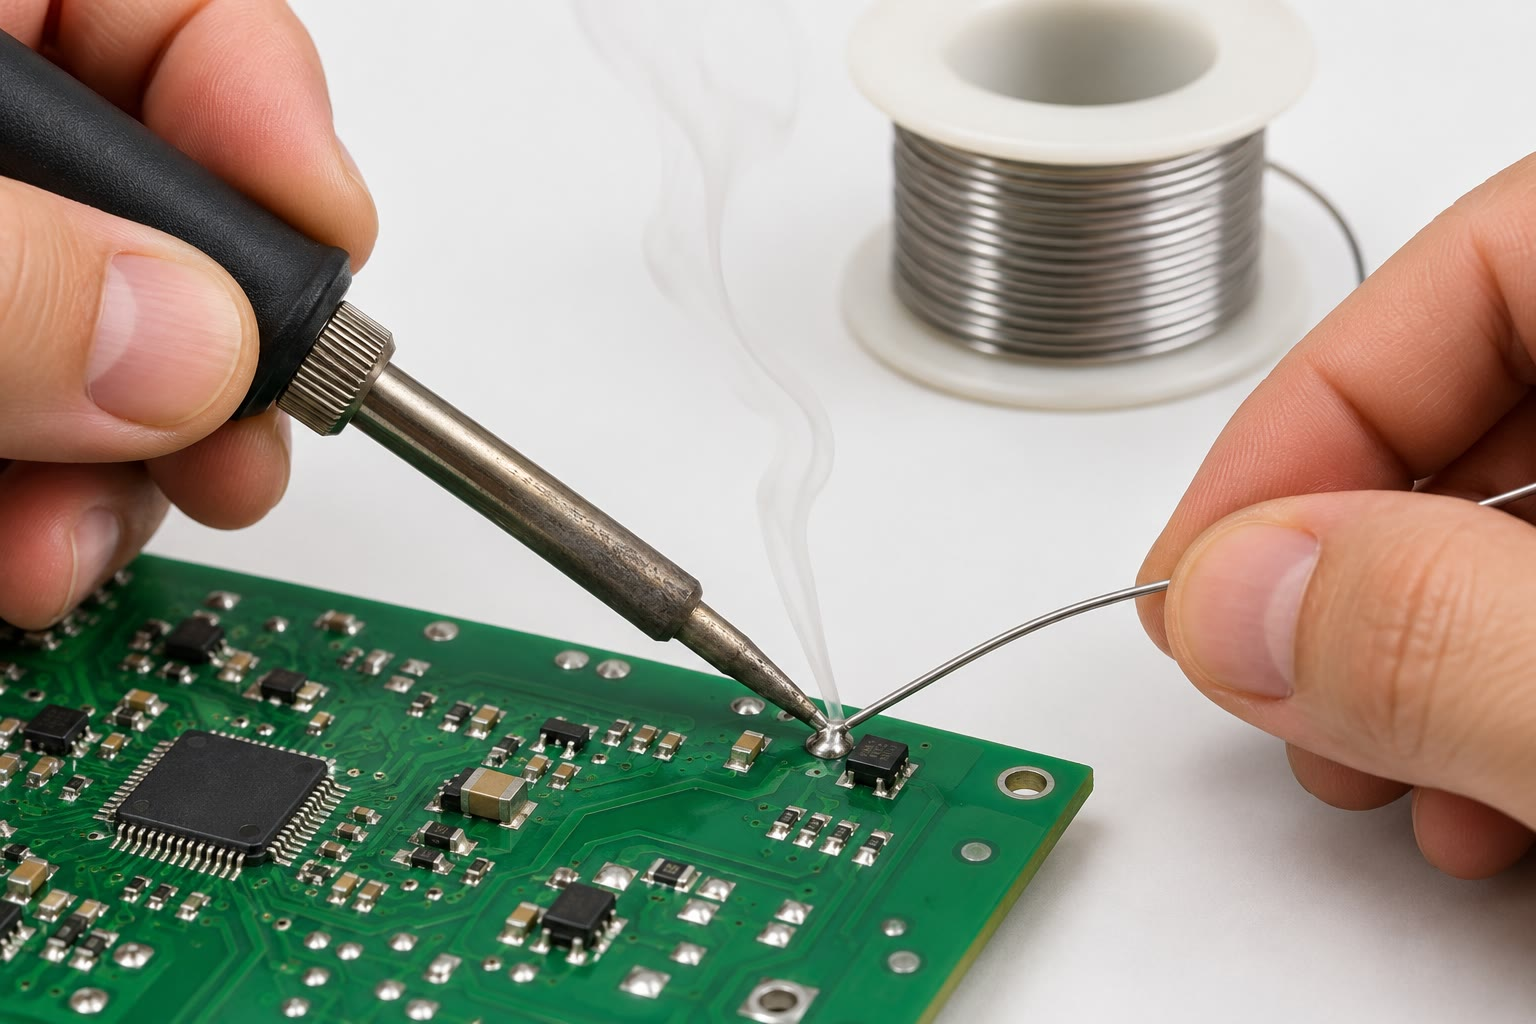
\includegraphics[width=0.6\linewidth]{images/book3/ai/b2-08-soldering.jpg}

{\small Menyolder sebuah komponen pada papan sirkuit: kawat solder melebur
ketika menyentuh solder yang panas, dan sambungannya membeku dalam satu
detik ketika solder itu diangkat --- karena paduannya melebur pada satu
suhu tunggal yang rendah.}
\end{omfigure}

\section{Analisis termal}

\begin{definition}[Analisis termal]\label{def:b2:solid-liquid-diagrams:cooling-curve}
Yang disebut \emph{analisis termal}\index{analisis termal} adalah penentuan
suhu-suhu perubahan wujud sebuah sampel dari suhunya yang direkam selama
sampel itu dipanaskan atau didinginkan dengan laju tetap. Rekaman suhu
terhadap waktu selama pendinginan yang lambat disebut \emph{kurva
pendinginan}\index{kurva pendinginan}.
\end{definition}

Jauh dari setiap perubahan wujud, sampel mendingin dengan mulus. Ketika
sebuah padatan mulai mengkristal, kalor kristalisasi memperlambat
pendinginan: kurvanya menunjukkan patahan kemiringan, atau berhenti pada
suhu tetap untuk sementara --- sebuah \textit{plato} --- jika pembekuan
terjadi pada suhu tetap.

\begin{proposition}[Plato]\label{prop:b2:solid-liquid-diagrams:plateaus}
Pada tekanan tetap, zat murni membeku pada suhu tetap, demikian pula
cairan biner yang darinya dua padatan mengkristal bersama. Cairan biner
yang darinya satu padatan mengkristal membeku dalam suatu rentang suhu.
\end{proposition}

\begin{proof}
Dengan tekanan yang ditetapkan, \omterm{def:b2:equilibrium-shifts:variance}{variansnya} adalah $v = n - r + 1 - \varphi$.
Zat murni, cair + padat: $v = 1 + 1 - 2 = 0$. Biner, cair + dua padatan:
$v = 2 + 1 - 3 = 0$. Biner, cair + satu padatan: $v = 2 + 1 - 2 = 1$: suhu
berubah seiring berubahnya komposisi cairan. \omterm{def:b2:equilibrium-shifts:variance}{Varians} 0 berarti suhu tidak
dapat berubah selama semua fase ada: kalor yang dibuang dipasok oleh
pembekuan, sampai sebuah fase lenyap.
\end{proof}

\begin{omfigure}
\begin{tikzpicture}[font=\small, x=0.55cm, y=0.05cm]
  \foreach \dx/\name in {0/logam murni, 9/{campuran, satu padatan lebih dulu}, 18/campuran eutektik} {
    \draw[->] (\dx,0) -- (\dx+7.5,0) node[below left, font=\scriptsize] {$t$};
    \draw[->] (\dx,0) -- (\dx,62) node[above, font=\scriptsize] {$T$};
    \node[font=\scriptsize] at (\dx+3.8,-8) {\name};
  }
  % pure: cool, plateau at 40, cool
  \draw[omDef, thick] (0,58) .. controls (1,48) and (1.6,42) .. (2,40) -- (4.5,40) .. controls (5.2,32) and (6,24) .. (7,20);
  \node[font=\scriptsize, anchor=south] at (3.25,40.5) {plato};
  % mixture: cool, break at 48, slow fall, plateau at 30, cool
  \draw[omDef, thick] (9,58) .. controls (9.6,53) and (9.9,50) .. (10.2,48)
     .. controls (11,42) and (11.6,35) .. (12.3,30) -- (14.2,30) .. controls (14.9,23) and (15.6,17) .. (16.5,14);
  \node[font=\scriptsize, anchor=west] at (10.4,49.5) {patahan};
  \node[font=\scriptsize, anchor=south] at (13.25,30.5) {eutektik};
  % eutectic: plateau at 30
  \draw[omDef, thick] (18,58) .. controls (19,46) and (19.8,36) .. (20.5,30) -- (24,30) .. controls (24.7,23) and (25.4,17) .. (26.2,14);
  \node[font=\scriptsize, anchor=south] at (22.25,30.5) {plato};
\end{tikzpicture}

{\small Kurva-kurva pendinginan, skematis. Logam murni membeku pada sebuah
plato. Campuran menunjukkan patahan kemiringan ketika padatan pertama
muncul, lalu pendinginan lambat cairan yang membeku dalam suatu rentang
suhu, lalu plato eutektik. Cairan dengan komposisi eutektik membeku pada
satu plato tunggal, seperti zat murni.}
\end{omfigure}

\begin{method}[Menyusun diagram dari kurva pendinginan]\label{met:b2:solid-liquid-diagrams:diagram-from-curves}
\begin{enumerate}
  \item Rekamlah \omterm{def:b2:solid-liquid-diagrams:cooling-curve}{kurva pendinginan} untuk serangkaian komposisi, termasuk
        komponen-komponen murni.
  \item Pada grafik (komposisi, suhu), alurkan untuk setiap komposisi suhu
        patahan pertama (awal kristalisasi) dan suhu setiap plato.
  \item Hubungkan titik-titik kristalisasi pertama: inilah \omterm{def:b2:solid-liquid-diagrams:liquidus}{likuidus}.
        Hubungkan titik-titik akhir pembekuan: \omterm{def:b2:solid-liquid-diagrams:liquidus}{solidus}. Plato yang
        ditemukan pada suhu yang sama untuk banyak komposisi adalah garis
        invarian (sebuah eutektik).
  \item Panjang plato eutektik, yang terbesar pada komposisi eutektik,
        menunjukkan letak komposisi itu.
\end{enumerate}
\end{method}

\section{Ketercampuran total dalam keadaan padat}

\begin{definition}[Larutan padat]\label{def:b2:solid-liquid-diagrams:solid-solution}
Yang disebut \emph{larutan padat}\index{larutan padat} adalah satu fase
kristal dengan komposisi yang dapat berubah-ubah, tempat atom-atom satu
komponen menggantikan atom-atom komponen yang lain pada situs-situs kisi
yang sama (substitusi) atau menempati rongga-rongga kisi itu
(interstisi).
\end{definition}

Tembaga dan nikel mempunyai struktur kubus berpusat muka yang sama dan
atom-atom dengan jari-jari yang berdekatan: keduanya membentuk \omterm{def:b2:solid-liquid-diagrams:solid-solution}{larutan padat}
substitusi pada setiap komposisi.

\begin{definition}[Likuidus dan solidus]\label{def:b2:solid-liquid-diagrams:liquidus}
Pada diagram padat--cair, yang disebut \emph{likuidus}\index{likuidus}
adalah kurva yang di atasnya semuanya cair; kurva ini memberikan komposisi
cairan yang berada dalam kesetimbangan dengan padatan. Yang disebut
\emph{solidus}\index{solidus} adalah kurva yang di bawahnya semuanya padat;
jika padatannya berupa larutan, kurva ini memberikan komposisi padatan yang
berada dalam kesetimbangan dengan cairan.
\end{definition}

\begin{proposition}[Lensa]\label{prop:b2:solid-liquid-diagrams:lens}
Jika kedua komponen membentuk larutan ideal dalam cairan dan dalam
padatan, \omterm{def:b2:solid-liquid-diagrams:liquidus}{likuidus} dan \omterm{def:b2:solid-liquid-diagrams:liquidus}{solidus} menghubungkan kedua titik lebur dan
melingkupi daerah dua fase berbentuk lensa; pada setiap suhu, fraksi mol
$x_i$ setiap komponen dalam cairan dan dalam padatan dihubungkan oleh
\[
  \frac{x_i^{\ell}}{x_i^{s}} = \exp\left[-\frac{\Delta_{\text{fus}}H_i}{R}\left(\frac1T - \frac1{T_i^*}\right)\right] .
\]
\end{proposition}

\begin{proof}
\omterm{def:b2:chemical-potential:chemical-potential}{Potensial kimia} $i$ sama dalam kedua fase, $\mu_i^{*,s} +
RT\ln x_i^s = \mu_i^{*,\ell} + RT\ln x_i^\ell$, sehingga
$RT\ln(x_i^\ell/x_i^s) =
-(\mu_i^{*,\ell} - \mu_i^{*,s}) = -\Delta_{\text{fus}}G_i(T)$, dan dengan $\Delta_{\text{fus}}H_i$ tetap,
$\Delta_{\text{fus}}G_i = \Delta_{\text{fus}}H_i(1 - T/T_i^*)$. Bersama
dengan $x_1 + x_2 = 1$ dalam setiap fase, kedua hubungan itu menetapkan
kedua komposisi pada setiap $T$ (diselesaikan secara numerik untuk
gambar); bahwa kurva-kurva yang dihasilkan membentuk lensa diterima tanpa
bukti.
\end{proof}

\begin{omfigure}
\begin{tikzpicture}
\begin{axis}[omphase, width=0.62\linewidth, height=7cm, ymin=1050, ymax=1480,
  xlabel={$x$ (nikel)}, ylabel={$T$ (\unit{\degreeCelsius})}]
\addplot[omliquidus] table[x=xl, y=T] {figdata/out/bachelor-2-solid-liquid-a.dat};
\addplot[omsolidus] table[x=xs, y=T] {figdata/out/bachelor-2-solid-liquid-a.dat};
\draw[tieline] (axis cs:0.541,1300) -- (axis cs:0.609,1300);
\fill (axis cs:0.58,1300) circle (1.3pt);
\node[font=\scriptsize] at (axis cs:0.25,1400) {cair};
\node[font=\scriptsize] at (axis cs:0.8,1150) {larutan padat};
\node[font=\scriptsize, anchor=east] at (axis cs:0.5,1330) {likuidus};
\node[font=\scriptsize, anchor=west] at (axis cs:0.66,1290) {solidus};
\node[font=\scriptsize, anchor=west] at (axis cs:0.03,1080) {\qty{1085}{\degreeCelsius}};
\draw[black!50] (axis cs:0.005,1084) -- (axis cs:0.03,1080);
\node[font=\scriptsize, anchor=south east] at (axis cs:1.0,1456) {\qty{1455}{\degreeCelsius}};
\end{axis}
\end{tikzpicture}

{\small Tembaga--nikel, dihitung untuk \omterm{def:b2:solid-liquid-diagrams:solid-solution}{larutan padat} dan larutan cair yang
ideal dari titik lebur dan entalpi peleburan kedua logam. Pada
\qty{1300}{\degreeCelsius}, paduan dengan komposisi 0.58 terbagi menjadi
cairan 0.541 dan padatan 0.609 (garis hubung putus-putus).}
% ledger: tfus:Cu, dfus:Cu, tfus:Ni, dfus:Ni
\end{omfigure}

\begin{method}[Membaca diagram padat--cair]\label{met:b2:solid-liquid-diagrams:read-solid-liquid}
\begin{enumerate}
  \item Ikutilah garis tegak komposisi keseluruhan ke bawah dari daerah
        cair.
  \item Pada \omterm{def:b2:solid-liquid-diagrams:liquidus}{likuidus}, padatan pertama muncul; komposisinya dibaca pada
        ujung lain garis hubung (\omterm{def:b2:solid-liquid-diagrams:liquidus}{solidus}, atau komponen murni).
  \item Dalam daerah dua fase, bacalah kedua komposisi pada ujung-ujung
        garis hubung dan proporsinya dengan \omterm{thm:b2:liquid-vapour-diagrams:lever}{aturan tuas}, dalam mol dengan
        fraksi mol, dalam massa dengan fraksi massa.
  \item Pada garis invarian mendatar, suhu berhenti sampai satu fase
        habis; di bawahnya, bacalah pasangan fase yang baru.
\end{enumerate}
\end{method}

\begin{example}[Sebuah paduan pada \qty{1300}{\degreeCelsius}]\label{ex:b2:solid-liquid-diagrams:lever}
Untuk paduan dengan fraksi mol nikel 0.58 pada \qty{1300}{\degreeCelsius},
fraksi atom yang berada dalam padatan adalah
$(0.58 - 0.541)/(0.609 - 0.541) = 0.57$. Padatan pertama yang muncul, di
dekat \qty{1315}{\degreeCelsius}, lebih kaya nikel daripada paduannya,
sedangkan cairan terakhir lebih miskin.
\end{example}

Diagram ini memerikan kesetimbangan, yang dalam padatan tercapai dengan
lambat: kristal-kristal pertama, yang kaya nikel, ditutupi oleh
lapisan-lapisan yang makin lama makin miskin nikel seiring berubahnya
cairan, dan difusi dalam padatan tidak sempat meratakannya. Coran yang
didinginkan dengan cepat terdiri atas kristal-kristal \textit{berlapis
inti}, yang komposisinya bergradasi dari pusat ke tepi; pemanasan lama di
bawah \omterm{def:b2:solid-liquid-diagrams:liquidus}{solidus} menghomogenkannya.

\section{Tanpa ketercampuran dalam keadaan padat: eutektik}

Jika kedua padatan sama sekali tidak bercampur, setiap komponen
mengkristal dalam keadaan murni, dan \omterm{def:b2:solid-liquid-diagrams:liquidus}{likuidus} mempunyai dua cabang, satu
untuk setiap padatan.

\begin{theorem}[Persamaan Schröder--van Laar]\label{thm:b2:solid-liquid-diagrams:schroder}
Jika komponen A mengkristal murni dari campuran cair ideal, \omterm{def:b2:solid-liquid-diagrams:liquidus}{likuidus} tempat
padatan A muncul diberikan oleh
\[
  \ln x_A = -\frac{\Delta_{\text{fus}}H_A}{R}\Big(\frac1T - \frac1{T_A^*}\Big),
\]
dengan $x_A$ fraksi mol A dalam cairan, $T_A^*$ dan $\Delta_{\text{fus}}H_A$
titik lebur dan entalpi peleburan A murni (yang dianggap tetap).
\end{theorem}

\begin{proof}
Pada kesetimbangan, \omterm{def:b2:chemical-potential:chemical-potential}{potensial kimia} A padat murni sama dengan \omterm{def:b2:chemical-potential:chemical-potential}{potensial
kimia} A dalam cairan: $\mu_A^{*,s}(T) = \mu_A^{*,\ell}(T) + RT\ln x_A$.
Jadi $R\ln x_A =
-\Delta_{\text{fus}}G_A(T)/T$. Menurut Gibbs--Helmholtz,
$d(\Delta_{\text{fus}}G_A/T)/
dT = -\Delta_{\text{fus}}H_A/T^2$; integrasi dari $T_A^*$, tempat
$\Delta_{\text{fus}}G_A = 0$, sampai $T$ memberikan
$\Delta_{\text{fus}}G_A/T =
\Delta_{\text{fus}}H_A(1/T - 1/T_A^*)$.
\end{proof}

Untuk larutan encer, $\ln x_A = \ln(1 - x_B) \approx -x_B$ dan
$1/T -
1/T_A^* \approx -\Delta T/T_A^{*2}$:
$\Delta T = RT_A^{*2}x_B/\Delta_{\text{fus}}H_A$, yaitu hukum krioskopi
pada \cref{ch:b2:chemical-potential}. Untuk benzena
($T^* =
\qty{278.64}{K}$, $\Delta_{\text{fus}}H = \qty{9.87}{kJ/mol}$,
$M =
\qty{78.11}{g/mol}$), \omterm{def:b2:chemical-potential:colligative}{tetapan krioskopik} $RT^{*2}M/\Delta_{\text{fus}}H$
bernilai \qty{5.11}{K.kg/mol}.
% ledger: tfus:benzene, dfus:benzene

\begin{definition}[Eutektik]\label{def:b2:solid-liquid-diagrams:eutectic}
Yang disebut \emph{titik eutektik}\index{titik eutektik} sebuah sistem
biner adalah titik tempat cairan berada dalam kesetimbangan dengan dua
padatan sekaligus; titik ini adalah suhu terendah tempat cairan masih ada
pada bagian diagram itu. Cairan dengan komposisi eutektik, dan campuran
halus dan akrab dua padatan yang terbentuk ketika cairan itu membeku,
disebut \emph{campuran eutektik}\index{campuran eutektik}.
\end{definition}

\begin{corollary}[Eutektik adalah tempat cabang-cabang likuidus bertemu]\label{cor:b2:solid-liquid-diagrams:eutectic}
Untuk dua komponen yang tidak bercampur dalam padatan dan ideal dalam
cairan, suhu eutektik $T_E$ dan komposisinya adalah penyelesaian
$x_A(T_E) + x_B(T_E) = 1$, dengan setiap $x$ diberikan oleh persamaan
Schröder--van Laar untuk padatannya sendiri.
\end{corollary}

\begin{proof}
Pada eutektik, cairan jenuh terhadap kedua padatan: cairan itu terletak
pada kedua cabang sekaligus, dengan komposisi yang sama baik dibaca dalam A
maupun dalam B.
\end{proof}

\begin{omfigure}
\begin{tikzpicture}
\begin{axis}[omphase, width=0.62\linewidth, height=6.5cm, ymin=-25, ymax=85,
  xlabel={$x$ (naftalena)}, ylabel={$T$ (\unit{\degreeCelsius})}]
\addplot[omliquidus] table[x=x, y=T] {figdata/out/bachelor-2-solid-liquid-b-benzene.dat};
\addplot[omliquidus] table[x=x, y=T] {figdata/out/bachelor-2-solid-liquid-b-naphthalene.dat};
\draw[thick] (axis cs:0,-3.55) -- (axis cs:1,-3.55);
\fill (axis cs:0.133,-3.55) circle (1.5pt);
\node[font=\scriptsize, anchor=north] at (axis cs:0.133,-4.5) {E};
\node[font=\scriptsize] at (axis cs:0.45,72) {cair};
\node[font=\scriptsize, align=center] at (axis cs:0.65,22) {cair + naftalena\\ padat};
\node[font=\scriptsize, anchor=south west] at (axis cs:0.08,45) {cair + benzena padat};
\draw[thin] (axis cs:0.12,45) -- (axis cs:0.06,0.8);
\node[font=\scriptsize] at (axis cs:0.55,-15) {benzena padat + naftalena padat};
\end{axis}
\end{tikzpicture}

{\small Benzena--naftalena, dihitung dengan persamaan Schröder--van Laar
untuk setiap padatan. Kedua cabang bertemu di eutektik E,
\qty{-3.5}{\degreeCelsius} dan 0.13 naftalena, yang di bawahnya semuanya
padat.}
% ledger: tfus:benzene, dfus:benzene, tfus:naphthalene, dfus:naphthalene
\end{omfigure}

\begin{example}[Mendinginkan campuran benzena--naftalena]\label{ex:b2:solid-liquid-diagrams:naphthalene}
Cairan dengan fraksi mol naftalena 0.5 mendingin sampai mencapai cabang
naftalena \omterm{def:b2:solid-liquid-diagrams:liquidus}{likuidus}, di dekat \qty{46}{\degreeCelsius}, tempat naftalena
padat murni mulai mengkristal. Cairan itu, yang kehilangan naftalena,
meluncur turun di sepanjang cabang itu; pada \qty{-3.5}{\degreeCelsius}
cairan itu mencapai eutektik, dan sisanya membeku pada suhu tetap menjadi
\omterm{def:b2:solid-liquid-diagrams:eutectic}{campuran eutektik}. Menurut \omterm{thm:b2:liquid-vapour-diagrams:lever}{aturan tuas}, tepat di atas eutektik, naftalena
padat merupakan $(0.5 - 0.133)/(1 - 0.133) =
42~\%$ dari jumlah mol, dan
cairan eutektik 58~\%.
\end{example}

\begin{proposition}[Panjang plato eutektik]\label{prop:b2:solid-liquid-diagrams:plateau-length}
Untuk sampel-sampel bermassa sama yang didinginkan dengan laju pembuangan
kalor yang sama, lamanya plato eutektik sebanding dengan jumlah cairan
yang mencapai eutektik, maksimum untuk komposisi eutektik dan nol untuk
komponen-komponen murni.
\end{proposition}

\begin{proof}
Pada plato, suhunya tetap: kalor yang dibuang, $\Phi\,\Delta t$ dengan laju
tetap $\Phi$, adalah kalor yang dilepaskan oleh pembekuan cairan eutektik,
$m_E\,\Delta_{\text{fus}}h_E$. Jadi $\Delta t = m_E\,\Delta_{\text{fus}}h_E/
\Phi$, sebanding dengan massa $m_E$ cairan eutektik, yang diberikan oleh
\omterm{thm:b2:liquid-vapour-diagrams:lever}{aturan tuas}.
\end{proof}

\section{Ketercampuran sebagian dan senyawa tertentu}

Sebagian besar pasangan logam tidak bercampur sempurna dan tidak pula sama
sekali tidak bercampur dalam keadaan padat: masing-masing melarutkan
sedikit yang lain. Timbal melarutkan timah sampai 19~\% massa, timah
melarutkan timbal sampai 3.4~\%. Diagramnya lalu memuat dua \omterm{def:b2:solid-liquid-diagrams:solid-solution}{larutan padat},
(Pb) dan (Sn), dan sebuah eutektik di antara keduanya; garis eutektik tidak
lagi mencapai sisi-sisi diagram, tetapi berhenti pada batas-batas \omterm{def:b2:solid-liquid-diagrams:solid-solution}{larutan
padat} itu.

\begin{omfigure}
\begin{tikzpicture}[font=\small, x=0.075cm, y=0.022cm]
  \draw[->] (0,0) -- (106,0) node[right] {\% Sn (massa)};
  \draw[->] (0,0) -- (0,360) node[above] {$T$ (\unit{\degreeCelsius})};
  \foreach \t in {100,200,300} \draw (0,\t) -- (-1.5,\t) node[left, font=\scriptsize] {\t};
  \foreach \w in {0,20,40,60,80,100} \draw (\w,0) -- (\w,-5) node[below, font=\scriptsize] {\w};
  % invariant points (NIST): Pb 327.5, Sn 231.9, eutectic 182.2 at 62.13; limits 18.91 and 96.59
  \draw[omliquidus] (0,327.5) .. controls (25,290) and (45,235) .. (62.13,182.2);
  \draw[omliquidus] (100,231.9) .. controls (85,215) and (72,200) .. (62.13,182.2);
  \draw[omsolidus] (0,327.5) .. controls (8,280) and (14,220) .. (18.91,182.2);
  \draw[omsolidus] (100,231.9) .. controls (98.5,215) and (97.5,200) .. (96.59,182.2);
  \draw[thick] (18.91,182.2) -- (96.59,182.2);
  \draw[omsolidus, densely dashed] (18.91,182.2) .. controls (12,120) and (6,60) .. (3,20);
  \draw[omsolidus, densely dashed] (96.59,182.2) .. controls (98.5,120) and (99.3,60) .. (99.6,20);
  \fill (62.13,182.2) circle (1.5pt);
  \fill (18.91,182.2) circle (1.2pt); \fill (96.59,182.2) circle (1.2pt);
  \node[anchor=south, font=\scriptsize] at (62.13,186) {E};
  \node[font=\scriptsize] at (55,300) {cair};
  \node[font=\scriptsize] at (6,150) {(Pb)};
  \node[font=\scriptsize] at (103,140) {(Sn)};
  \node[font=\scriptsize] at (28,235) {L + (Pb)};
  \node[font=\scriptsize] at (84,192) {L + (Sn)};
  \node[font=\scriptsize] at (55,100) {(Pb) + (Sn)};
  % cooling path at 40 %
  \draw[->, omProp, thick] (40,340) -- (40,30);
  \node[font=\scriptsize, omProp, anchor=south] at (40,342) {40~\%};
  \node[font=\scriptsize, anchor=north east] at (16.6,179) {18.9};
  \node[font=\scriptsize, anchor=north] at (62.13,178) {62.1};
  \node[font=\scriptsize, anchor=north east] at (95.8,178) {96.6};
  \node[font=\scriptsize, anchor=west] at (101,182.2) {\qty{182.2}{\degreeCelsius}};
\end{tikzpicture}

{\small Diagram timbal--timah, yang digambar melalui titik-titik
invariannya: titik lebur timbal (\qty{327.5}{\degreeCelsius}) dan timah
(\qty{231.9}{\degreeCelsius}), eutektik E pada \qty{182.2}{\degreeCelsius}
dan 62.1~\% timah, batas-batas \omterm{def:b2:solid-liquid-diagrams:solid-solution}{larutan padat} pada suhu eutektik (18.9~\%
dan 96.6~\% timah). Kurva-kurva di antara titik-titik itu, dan batas
kelarutan putus-putus di bawah eutektik, digambar secara skematis. Panah:
pendinginan solder 40~\%.}
% ledger: eut:Pb-Sn.T, eut:Pb-Sn.wL, eut:Pb-Sn.wPb, eut:Pb-Sn.wSn, tfus:Pb, tfus:Sn
\end{omfigure}

Solder dengan 40~\% timah mulai membeku pada \omterm{def:b2:solid-liquid-diagrams:liquidus}{likuidus} dengan mengendapkan
kristal-kristal larutan yang kaya timbal (Pb); cairannya makin kaya timah
sampai, pada \qty{182.2}{\degreeCelsius}, mencapai komposisi eutektik dan
membeku menjadi campuran halus lamela (Pb) dan (Sn), di sekeliling
kristal-kristal primer.

\begin{omfigure}
\begin{tikzpicture}[font=\small]
  \begin{scope}
    \clip (0,0) circle (2.2);
    \fill[gray!20] (-2.3,-2.3) rectangle (2.3,2.3);
    \foreach \k in {-24,...,24} \draw[gray!65, line width=1.1pt] (-2.4+0.2*\k,-2.4) -- ++(55:6);
    \foreach \cx/\cy/\r/\a in {-0.9/0.8/0.55/10, 0.7/1.0/0.45/40, 0.2/-0.6/0.6/-20, -1.1/-0.9/0.4/70, 1.3/-0.3/0.35/5} {
      \fill[omDef!35, draw=omDef, rotate around={\a:(\cx,\cy)}] (\cx,\cy) ellipse ({\r} and {0.7*\r});
    }
  \end{scope}
  \draw[thick] (0,0) circle (2.2);
  \draw[<-, omProp, thick] (0.7,1.0) -- (3.0,1.6) node[right, text=black] {kristal (Pb) primer};
  \draw[<-, omProp, thick] (1.6,0.9) -- (3.0,0.5) node[right, text=black, align=left] {eutektik: lamela (Pb)\\ dan (Sn) berselang-seling};
\end{tikzpicture}

{\small Mikrostruktur solder dengan 40~\% timah setelah pendinginan lambat,
skematis: kristal-kristal primer (Pb), yang terbentuk di antara \omterm{def:b2:solid-liquid-diagrams:liquidus}{likuidus}
dan eutektik, di dalam matriks eutektik yang terdiri atas pelat-pelat
tipis kedua \omterm{def:b2:solid-liquid-diagrams:solid-solution}{larutan padat} yang berselang-seling.}
\end{omfigure}

\begin{definition}[Senyawa tertentu]\label{def:b2:solid-liquid-diagrams:defined-compound}
Yang disebut \emph{senyawa tertentu}\index{senyawa tertentu} adalah padatan
dengan komposisi tetap $\mathrm{A}_a\mathrm{B}_b$ yang dibentuk oleh kedua
komponen. Senyawa itu menunjukkan \emph{peleburan
kongruen}\index{peleburan kongruen} jika melebur menjadi cairan dengan
komposisinya sendiri: \omterm{def:b2:solid-liquid-diagrams:liquidus}{likuidus} lalu mempunyai maksimum pada komposisi itu.
\end{definition}

Senyawa dengan \omterm{def:b2:solid-liquid-diagrams:defined-compound}{peleburan kongruen} membagi diagram menjadi dua: setiap
paruhnya, A dengan $\mathrm{A}_a\mathrm{B}_b$ dan $\mathrm{A}_a\mathrm{B}_b$
dengan B, adalah diagram tersendiri, dengan eutektiknya sendiri. Komposisi
maksimum, yang dibaca dalam fraksi mol, memberikan rumus senyawa itu.

\begin{omfigure}
\begin{tikzpicture}[font=\small, x=6cm, y=0.05cm]
  \draw[->] (0,0) -- (1.06,0) node[right] {$x_{\mathrm B}$};
  \draw[->] (0,0) -- (0,95) node[above] {$T$};
  \node[below, font=\scriptsize] at (0,0) {A}; \node[below, font=\scriptsize] at (1,0) {B};
  \node[below, font=\scriptsize] at (0.667,0) {$\tfrac23$};
  \draw[omliquidus] (0,70) .. controls (0.12,58) and (0.25,45) .. (0.35,35);
  \draw[omliquidus] (0.35,35) .. controls (0.45,62) and (0.58,79) .. (0.667,80);
  \draw[omliquidus] (0.667,80) .. controls (0.75,79) and (0.8,68) .. (0.85,50);
  \draw[omliquidus] (0.85,50) .. controls (0.9,56) and (0.95,62) .. (1,65);
  \draw[thick] (0,35) -- (0.667,35); \draw[thick] (0.667,50) -- (1,50);
  \draw[thick] (0.667,0) -- (0.667,80);
  \fill (0.35,35) circle[radius=1.5pt]; \fill (0.85,50) circle[radius=1.5pt];
  \fill (0.667,80) circle[radius=1.5pt];
  \node[anchor=north, font=\scriptsize] at (0.35,34) {E$_1$};
  \node[anchor=north, font=\scriptsize] at (0.85,49) {E$_2$};
  \node[anchor=south, font=\scriptsize] at (0.667,81) {$\mathrm{AB_2}$ melebur};
  \node[font=\scriptsize] at (0.35,80) {cair};
  \node[font=\scriptsize, align=center] at (0.33,15) {A +\\ $\mathrm{AB_2}$};
  \node[font=\scriptsize, align=center] at (0.84,25) {$\mathrm{AB_2}$\\ + B};
\end{tikzpicture}

{\small Diagram skematis dengan \omterm{def:b2:solid-liquid-diagrams:defined-compound}{senyawa tertentu} $\mathrm{AB_2}$ (garis tegak
pada $x_{\mathrm B} = 2/3$) yang melebur secara kongruen pada maksimum
\omterm{def:b2:solid-liquid-diagrams:liquidus}{likuidus}. Diagram ini terdiri atas dua diagram eutektik sederhana yang
berdampingan, dengan eutektik E$_1$ dan E$_2$.}
\end{omfigure}

\section{Penerapan}

\paragraph{Solder dan paduan bertitik lebur rendah.} Solder harus melebur
di bawah titik lebur bagian-bagian yang disambungkannya dan membeku dengan
cepat, tanpa rentang lembek: komposisi eutektik adalah pilihan yang wajar.
Eutektik timah--timbal melebur pada \qty{182.2}{\degreeCelsius}; karena
timbal beracun, elektronika kini memakai solder bebas timbal, di
antaranya eutektik bismut--timah, yang melebur pada
\qty{138.8}{\degreeCelsius} dan mengandung 57~\% massa bismut.
% ledger: eut:Pb-Sn.T, eut:Bi-Sn.T, eut:Bi-Sn.wL

\paragraph{Pencairan es.} Es dan garam membentuk eutektik: eutektik es--garam
dihidrat terletak pada \qty{252}{K} (\qty{-21}{\degreeCelsius}) dan
23.3~\% massa natrium klorida. Di atas suhu itu, garam yang bersentuhan
dengan es membentuk air garam yang titik bekunya di bawah suhu jalan, dan
es mencair; di bawahnya, tidak ada cairan yang dapat ada, dan garam tidak
berguna.
% ledger: eut:NaCl-water.T, eut:NaCl-water.w

\paragraph{Kristalisasi.} Diagram sebuah garam dan air dibaca seperti
diagram lainnya: pendinginan larutan jenuh yang panas melintasi kurva
kelarutan (\omterm{def:b2:solid-liquid-diagrams:liquidus}{likuidus} garam itu), dan kristal-kristal murni garam itu
mengendap sementara pengotor, yang terlalu encer untuk mencapai
\omterm{def:b2:solid-liquid-diagrams:liquidus}{likuidusnya} sendiri, tetap berada dalam larutan induk. Inilah pemurnian
dengan rekristalisasi dari jilid Tahun 1, dilihat pada sebuah diagram.

\begin{omfigure}
\begin{tikzpicture}
\begin{axis}[omphase, width=0.62\linewidth, height=6cm, xmin=0, xmax=100,
  ymin=90, ymax=285, xlabel={\% Bi (massa)}, ylabel={$T$ (\unit{\degreeCelsius})}]
\addplot[omliquidus] table[x=w, y=T] {figdata/out/bachelor-2-solid-liquid-d-Sn.dat};
\addplot[omliquidus] table[x=w, y=T] {figdata/out/bachelor-2-solid-liquid-d-Bi.dat};
\draw[densely dashed] (axis cs:0,119.5) -- (axis cs:100,119.5);
\fill[omThm] (axis cs:56.97,138.8) circle (2pt);
\node[font=\scriptsize, omThm, anchor=west] at (axis cs:64,129) {eutektik terkaji};
\draw[omThm, thin] (axis cs:64,129) -- (axis cs:57.8,137.6);
\node[font=\scriptsize, anchor=north] at (axis cs:52,118) {model ideal};
\node[font=\scriptsize] at (axis cs:50,250) {cair};
\end{axis}
\end{tikzpicture}

{\small Bismut--timah: \omterm{def:b2:solid-liquid-diagrams:liquidus}{likuidus} yang diramalkan untuk padatan murni dan
cairan ideal (Schröder--van Laar, biru) bertemu pada eutektik di dekat
\qty{120}{\degreeCelsius}; eutektik terkaji (titik merah) terletak pada
\qty{138.8}{\degreeCelsius} dan 57~\% bismut.}
% ledger: tfus:Sn, dfus:Sn, tfus:Bi, dfus:Bi, eut:Bi-Sn.T, eut:Bi-Sn.wL
\end{omfigure}

\section{Latihan}

\begin{exercise}[$\star$]\label{exo:b2:solid-liquid-diagrams:1}
Pada diagram tembaga--nikel, berikan fase-fase yang ada pada
\qty{1300}{\degreeCelsius} untuk fraksi mol nikel 0.40, 0.58, dan 0.70.
\end{exercise}

\begin{exercise}[$\star$]\label{exo:b2:solid-liquid-diagrams:2}
Sebanyak \qty{2.00}{mol} paduan tembaga--nikel dengan fraksi mol nikel 0.58
dijaga pada \qty{1300}{\degreeCelsius}. Hitunglah jumlah padatan dan
cairan serta jumlah nikel dalam masing-masing.
\end{exercise}

\begin{exercise}[$\star$]\label{exo:b2:solid-liquid-diagrams:3}
Hitunglah \omterm{def:b2:equilibrium-shifts:variance}{varians} pada tekanan tetap (a) logam murni ketika membeku;
(b) paduan tembaga--nikel ketika membeku; (c) cairan timbal--timah pada
garis eutektik.
\end{exercise}

\begin{exercise}[$\star$]\label{exo:b2:solid-liquid-diagrams:4}
Sketsalah \omterm{def:b2:solid-liquid-diagrams:cooling-curve}{kurva pendinginan} timah murni dari \qty{300}{\degreeCelsius}
sampai \qty{100}{\degreeCelsius} dan jelaskan mengapa suhunya berhenti
pada \qty{232}{\degreeCelsius}.
\end{exercise}

\begin{exercise}[$\star\star$]\label{exo:b2:solid-liquid-diagrams:5}
Dengan data dalam bab ini (benzena \qty{278.64}{K}, \qty{9.87}{kJ/mol};
naftalena \qty{353.2}{K}, \qty{19.1}{kJ/mol}), periksalah bahwa pada
\qty{269.6}{K} kedua fraksi mol Schröder--van Laar berjumlah 1, lalu
berikan komposisi eutektiknya.
\end{exercise}

\begin{exercise}[$\star\star$]\label{exo:b2:solid-liquid-diagrams:6}
Uraikan pendinginan paduan timbal--timah dengan 30~\% massa timah, dari
cairan sampai suhu kamar, lalu hitunglah fraksi massa eutektik yang
dikandungnya.
\end{exercise}

\begin{exercise}[$\star\star$]\label{exo:b2:solid-liquid-diagrams:7}
Berapa massa natrium klorida per kilogram air yang dikandung air garam
eutektik? Mengapa menaburkan garam di jalan tidak berguna pada
\qty{-25}{\degreeCelsius}?
\end{exercise}

\begin{exercise}[$\star\star$]\label{exo:b2:solid-liquid-diagrams:8}
Pada diagram skematis dengan senyawa $\mathrm{AB_2}$, uraikan pendinginan
cairan dengan $x_{\mathrm B} = 0.5$ dan $x_{\mathrm B} = 0.9$: padatan
pertama, eutektik yang dicapai, dan padatan pada akhirnya.
\end{exercise}

\begin{exercise}[$\star\star$]\label{exo:b2:solid-liquid-diagrams:9}
Dalam pemurnian zona, sebuah zona leleh digerakkan perlahan-lahan di
sepanjang batang. Di dekat nikel murni, rasio fraksi mol tembaga dalam
padatan dan dalam cairan pada kesetimbangan sekitar 0.78. Jelaskan
mengapa tembaga terbawa bersama zona leleh, dan mengapa diperlukan
beberapa kali lintasan.
\end{exercise}

\begin{exercise}[$\star\star\star$]\label{exo:b2:solid-liquid-diagrams:10}
Turunkan persamaan Schröder--van Laar, lalu tunjukkan bahwa untuk cairan
encer persamaan itu tereduksi menjadi $\Delta T = K_f\,b$, dengan
$K_f = RT^{*2}M_A/\Delta_{\text{fus}}H_A$ dan $b$ molalitas zat terlarut;
hitunglah $K_f$ untuk benzena.
\end{exercise}

\begin{exercise}[$\star\star\star$]\label{exo:b2:solid-liquid-diagrams:11}
Diagram magnesium--timbal mempunyai maksimum \omterm{def:b2:solid-liquid-diagrams:liquidus}{likuidus} pada 19.0~\% massa
magnesium. Tentukan rumus senyawanya.
\end{exercise}

\begin{exercise}[$\star\star\star$]\label{exo:b2:solid-liquid-diagrams:12}
Paduan-paduan timbal--timah bermassa sama didinginkan dalam kondisi yang
sama. Paduan eutektik menunjukkan plato selama \qty{300}{s}; sebuah paduan
yang tidak diketahui menunjukkan plato selama \qty{120}{s}. Tentukan kedua
komposisi yang mungkin untuk paduan itu, lalu jelaskan cara membedakan
keduanya.
\end{exercise}

\section{Soal: Solder}

\begin{problem}[{Soal akhir pekan --- diagram timbal--timah dari
titik-titik invariannya, pembekuan solder 40~\% dengan aturan tuas,
solder bismut--timah bebas timbal yang diramalkan oleh model cairan ideal,
dan pemilihan solder}]
\label{pb:b2:solid-liquid-diagrams:1}
Data (NIST, kesetimbangan invarian terhitung): eutektik timbal--timah pada
\qty{182.2}{\degreeCelsius}, cairan dengan 62.13~\% massa timah, dalam
kesetimbangan dengan (Pb) 18.91~\% dan (Sn) 96.59~\% timah; eutektik
bismut--timah pada \qty{138.8}{\degreeCelsius}, cairan dengan 56.97~\%
bismut. Titik lebur dan entalpi peleburan: timbal \qty{600.6}{K},
\qty{4.77}{kJ/mol}; timah \qty{505.1}{K}, \qty{7.03}{kJ/mol}; bismut
\qty{544.6}{K}, \qty{11.30}{kJ/mol}. Massa molar (\unit{g/mol}): Pb 207.2,
Sn 118.71, Bi 208.98.
% ledger: eut:Pb-Sn.T, eut:Pb-Sn.wL, eut:Pb-Sn.wPb, eut:Pb-Sn.wSn, eut:Bi-Sn.T, eut:Bi-Sn.wL, tfus:Pb, dfus:Pb, tfus:Sn, dfus:Sn, tfus:Bi, dfus:Bi, aw:Pb, aw:Sn, aw:Bi

\medskip
\noindent\textbf{Bagian I --- Diagram timbal--timah.}
\begin{enumerate}
  \item Ubahlah titik lebur timbal dan timah ke derajat Celsius.
  \item Ubahlah komposisi eutektik menjadi fraksi mol timah.
  \item Letakkan pada grafik (\% massa Sn, $T$) titik-titik lebur,
        eutektik, dan kedua ujung garis eutektik.
  \item Gambarlah diagramnya dan namai keenam daerahnya.
  \item Tuliskan transformasi eutektik pada pendinginan.
  \item Hitunglah \omterm{def:b2:equilibrium-shifts:variance}{varians} pada garis eutektik pada tekanan tetap.
\end{enumerate}

\medskip
\noindent\textbf{Bagian II --- Mendinginkan solder 40~\%.}
\begin{enumerate}[resume]
  \item Padatan mana yang muncul pertama, dan mengapa padatan itu bukan
        timbal murni?
  \item Bagaimana komposisi cairan berubah selama pendinginan sampai
        eutektik?
  \item Tepat di atas \qty{182.2}{\degreeCelsius}: fase-fase apa, dengan
        komposisi berapa?
  \item Hitunglah fraksi massanya.
  \item Tepat di bawahnya: fase-fase apa, dengan komposisi berapa, dan
        dalam fraksi massa berapa?
  \item Berapa bagian paduan yang terdiri atas konstituen eutektik, dan
        berapa bagian kristal (Pb) primer?
  \item Sketsalah \omterm{def:b2:solid-liquid-diagrams:cooling-curve}{kurva pendinginannya} dan bandingkan platonya dengan plato
        paduan eutektik.
\end{enumerate}

\medskip
\noindent\textbf{Bagian III --- Solder bebas timbal menurut model cairan ideal.}
\begin{enumerate}[resume]
  \item Tuliskan persamaan Schröder--van Laar untuk \omterm{def:b2:solid-liquid-diagrams:liquidus}{likuidus} timah.
  \item Tuliskan persamaan itu untuk \omterm{def:b2:solid-liquid-diagrams:liquidus}{likuidus} bismut.
  \item Tuliskan syarat yang mendefinisikan eutektik.
  \item Hitunglah jumlah kedua fraksi mol pada \qty{110}{\degreeCelsius},
        \qty{120}{\degreeCelsius}, dan \qty{130}{\degreeCelsius}, lalu
        tentukan suhu eutektik model itu sampai derajat terdekat.
  \item Berikan komposisi eutektik model itu, dalam fraksi mol dan fraksi
        massa bismut.
  \item Bandingkan dengan eutektik terkaji.
  \item Timah melarutkan bismut sampai 21~\% dalam keadaan padat. Jelaskan
        bagaimana hal ini membuat eutektik yang sebenarnya lebih panas
        daripada eutektik model.
\end{enumerate}

\medskip
\noindent\textbf{Bagian IV --- Memilih solder.}
\begin{enumerate}[resume]
  \item Mengapa komposisi eutektik lebih disukai untuk solder?
  \item Berikan satu alasan untuk mengganti timbal dalam solder.
  \item Apa yang ditawarkan oleh titik lebur rendah eutektik bismut--timah,
        dan apa yang mungkin menjadi harganya?
  \item Hitunglah massa bismut dan timah dalam \qty{1.00}{kg} solder
        eutektik bismut--timah.
  \item Nyatakan suhu eutektik bismut--timah yang diramalkan oleh model
        cairan ideal.
\end{enumerate}
\end{problem}
